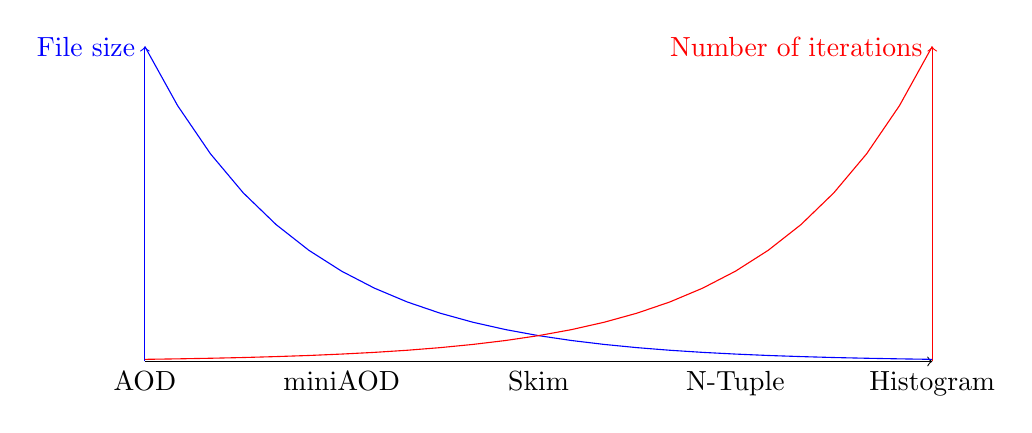
\begin{tikzpicture}[scale=1.0]
% horizontal axis
\draw[->] (0,0) -- (10,0) node[anchor=north] {};
% vertical axis
\draw[blue,->] (0,0) -- (0,4) node[anchor=east] {File size};
\draw[red,->] (10,0) -- (10,4) node[anchor=east] {Number of iterations};
% file size
\draw[blue,domain=0:10] plot (\x,{4*exp(-\x/2)});
\draw[red,domain=0:10] plot (\x,{4*exp((\x-10)/2)});
% labels
\draw	(0,0) node[anchor=north] {AOD}
		(2.5,0) node[anchor=north] {miniAOD}
		(5,0) node[anchor=north] {Skim}
		(7.5,0) node[anchor=north] {N-Tuple}
		(10,0) node[anchor=north] {Histogram};
\end{tikzpicture}
